\newpage
\section{Plano de desenvolvimento da aplicação}

	Implementamos e desenvolvemos essa aplicação durante nosso estudo com processamento de imagens e OCR (reconhecimento ótico de caracteres). Já está conseguindo reconhecer palavras completas com espaços e quebra de linhas. Assim conseguimos reconhecer qualquer letra ou palavras do nosso alfabeto, nosso projeto foi desenvolvido com o intuito de utilizar duas matérias muito importantes durante esse 6º módulo, que são Processamento de Imagem, e Sistema de Informação Inteligentes, dessas matérias retiramos conhecimento para o desenvolvimento dessa aplicação. 
	
	A ideia é fazer o sistema reconhecer letras e palavras do alfabeto escrita a mão, para que funcionasse perfeitamente treinamos uma imagem do nosso alfabeto escrito a mão. Para que a aplicação aprenda todas as letras, e reconheça as palavras que forem escritas a mão, toda vez que quisermos que o sistema entenda uma palavra diferente, precisamos treiná-la, para que o sistema aprenda e com isso reconheça a palavra na imagem. O processo para que a aplicação leia a palavra, começa quando recortamos as letras do alfabeto que o sistema já reconhece e formamos a palavra, importamos para o programa para treiná-la, após o treinamento, pedimos para o sistema reconhecer a palavra que está na imagem, ele reconhece a palavra corretamente. Qualquer letra ou palavra do alfabeto que for colocado no sistema para reconhecimento, será reconhecida, no log do projeto é visualizado letra por letra a porcentagem de aprendizado do programa, assim verificamos como se fosse um gráfico para o aprendizado de cada letra que o programa teve, podendo ter uma ideia da qualidade do sistema que foi desenvolvido, até o momento todas palavras e letras foram reconhecidas com êxito. 

\begin{figure}[!htb]
	\centering
	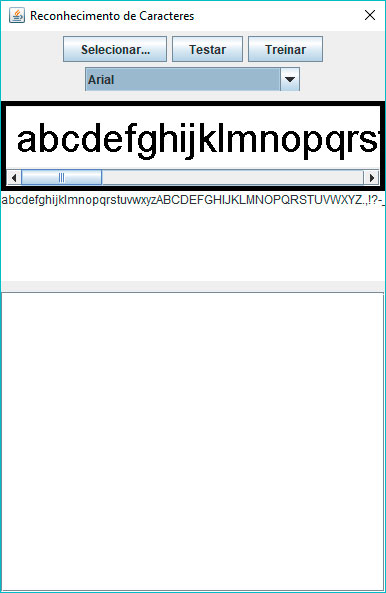
\includegraphics[scale=0.5]{img/01-reconhecimento-letras-basicas.jpg}
	\caption{Reconhecimento de letras básicas}
	\label{Reconhecimento}
\end{figure}